\documentclass[12pt]{article}

\usepackage[utf8]{inputenc}
\usepackage[english]{babel}
\usepackage{amssymb}
\usepackage{amsfonts}
\usepackage{amsmath}
\usepackage{graphicx}
\usepackage[margin=1in]{geometry}
\usepackage[hidelinks]{hyperref}
\usepackage{float}
\usepackage[danish]{varioref}
\usepackage{multirow}
\usepackage{hhline}
\usepackage{inconsolata}
\usepackage{etoolbox}
\usepackage[usenames,dvipsnames]{xcolor}
\usepackage{tikz}
\usetikzlibrary{positioning,shapes, shadows, arrows}
\usepackage{listings}

\setlength\parindent{0pt}
\usepackage[parfill]{parskip}

\definecolor{dark-blue}{HTML}{000080}
\definecolor{dark-green}{HTML}{008000}
\definecolor{pale-purple}{HTML}{94558D}
\definecolor{dark-purple}{HTML}{0000AA}
\definecolor{regular-purple}{HTML}{660099}
\definecolor{magenta}{HTML}{B200B2}
\definecolor{light-gray}{HTML}{FAFAFA}
\definecolor{dark-gray}{HTML}{2D2D2D}
\definecolor{comment}{HTML}{808080}
\definecolor{digit}{HTML}{0000FF}

\newcommand*{\FormatDigit}[1]{\textcolor{digit}{#1}}

\lstset{
	language=Python,
	prebreak=\raisebox{0ex}[0ex][0ex]{\ensuremath{\color{red}\space\hookleftarrow}},
	basicstyle=\footnotesize\ttfamily,
	%
	literate=%
    	{0}{{\FormatDigit{0}}}{1}%
        {1}{{\FormatDigit{1}}}{1}%
        {2}{{\FormatDigit{2}}}{1}%
        {3}{{\FormatDigit{3}}}{1}%
        {4}{{\FormatDigit{4}}}{1}%
        {5}{{\FormatDigit{5}}}{1}%
        {6}{{\FormatDigit{6}}}{1}%
        {7}{{\FormatDigit{7}}}{1}%
        {8}{{\FormatDigit{8}}}{1}%
        {9}{{\FormatDigit{9}}}{1}%
        {.0}{{\FormatDigit{.0}}}{2}% Following is to ensure that only periods
        {.1}{{\FormatDigit{.1}}}{2}% followed by a digit are changed.
        {.2}{{\FormatDigit{.2}}}{2}%
        {.3}{{\FormatDigit{.3}}}{2}%
        {.4}{{\FormatDigit{.4}}}{2}%
        {.5}{{\FormatDigit{.5}}}{2}%
        {.6}{{\FormatDigit{.6}}}{2}%
        {.7}{{\FormatDigit{.7}}}{2}%
        {.8}{{\FormatDigit{.8}}}{2}%
        {.9}{{\FormatDigit{.9}}}{2}%
        %{,}{{\FormatDigit{,}}{1}% depends if you want the "," in color
        {\ }{{ }}{1}% handle the space
		{æ}{{\ae}}1
        {ø}{{\o}}1
        {å}{{\aa}}1
        {Æ}{{\AE}}1	
        {Ø}{{\O}}1
        {Å}{{\AA}}1,
	%
	%emph={},
	otherkeywords={},
	keywords=[2]{self},
	keywords=[3]{__init__},
	keywords=[4]{object},
	keywords=[5]{encoding, flags},
	keywords=[6]{reduce,list,enumerate,len,map,range,sorted,None,super,@staticmethod},
	%
	keywordstyle=\bfseries\color{dark-blue},
	keywordstyle={[2]\color{pale-purple}},
	keywordstyle={[3]\color{magenta}},
	keywordstyle={[4]\color{dark-blue}},
	keywordstyle={[5]\color{regular-purple}},
	keywordstyle={[6]\color{dark-purple}},
    commentstyle=\itshape\color{comment},
    identifierstyle=\color{black},
	stringstyle=\bfseries\color{dark-green},
	%emphstyle=\color{dark-purple},
	%
	numbers=left, % where to put the line-numbers
	numberstyle=\ttfamily\color{dark-gray},
	numbersep=5pt, % how far the line-numbers are from the code
	stepnumber=1,
	showstringspaces=false,
	backgroundcolor=\color{light-gray},
	tabsize=4,
	captionpos=b, % sets the caption-position to bottom
	breaklines=true % sets automatic line breaking
}

\linespread{1.3}

\begin{document}

\begin{titlepage}
    \vspace*{\fill}
    \begin{center}
      {\Huge Synopsis for Bachelorproject}\\[0.7cm]
      {\Large Regular Expression Matching In Genomic Data}\\[0.4cm]
      {\large Rasmus Haarslev - nkh877}\\
      {\large Troels Thomsen - qvw203}\\[0.4cm]
      {Supervisors: Rasmus Fonseca}\\
      {\small 23. Februar 2015}\\[0.3cm] 
      {\small Department of Computer Science}\\
      {\small University of Copenhagen}
    \end{center}
    \vspace*{\fill}
\end{titlepage}	

\clearpage

\thispagestyle{empty}

\newpage

\section{Problem definition}

We wish to determine the possibility of converting sequence analysis patterns used for scan-for-matches\cite{scan-for-matches}, into regular expressions\cite{crash-course-regex} and test their efficiency against the KMC\cite{kmc-website} engine.

Specifically we wish to solve the following problems:

\begin{itemize}
	\item Is it possible to programatically convert patterns used by the scan-for-matches program into regular expressions for the KMC engine? If not all patterns used by scan-for-matches then which ones?
	\item Is it possible to achieve speeds matching or exceeding scan-for-matches with the generated regular expressions and the KMC engine?
	\item Can we find weak extensions to regular expressions, which would enable us to support more or all scan-for-matches patterns?
\end{itemize}

\subsection{Limits}

\begin{itemize}
	\item We will not attempt to modify the KMC engine.
	\item We will not look into the theory behind the scan-for-matches engine.
\end{itemize}

\newpage

\section{Motivation}

Institute for Microbiology have a allocated, and are still allocating, a lot of DNA sequencing data. Currently they have around a total of 2 petabytes of data. These sequences of DNA contain a lot of information, but searching through the data currently uses the scan-for-matches program, which while performing very well, is not very user friendly and have some unfortunate limitations when running many consecutive scans, since it performs I/O operations for every run.

Recently, Professor Henglein's group have developed a regular expression engine called KMC, which so far have performed five times better than current industry standard engines. Since scan-for-matches outperforms NR-grep\cite{nrgrep}, we are hoping that optimized regular expressions running on KMC will be able to outperform NR-grep and subsequently scan-for-matches.

If we could achieve a performance improvement over scan-for-matches, it would greatly benefit the bioinformatics team. As such we see this as a chance to make a unique contribution to ongoing and future research projects, while at the same time providing a chance for the KMC team to have their engine tested in a new scenario.

\newpage

\section{Tasks and Schedule}

\begin{itemize}
	\item Develop a standalone Ruby and C application as a solution to the tasks defined in the problem definition.
	\begin{itemize}
		\item \textbf{Product:} A fully functional Ruby/C application, that can translate scan-for-matches patterns into regular expressions, understood by the KMC engine.
		\item \textbf{Resource demands:} Laptops, our contact persons with insight in the KMC engine, testing data in the fasta format, and the KMC engine.
		\item \textbf{Dependencies:} Problem definition
		\item \textbf{Time demands:} 5 weeks
	\end{itemize}
	
	\item Test and analyze the efficiency of our regular expressions on the KMC engine, compared to scan-for-matches.
	\begin{itemize}
		\item \textbf{Product:} An extensive analyzis of our regular expressions in combination with the KMC engine, with suggestions for possible improvements.
		\item \textbf{Resource demands:} Laptops, testing data in the fasta format, and the KMC engine.
		\item \textbf{Dependencies:} The application that we developed.
		\item \textbf{Time demands:} 5 weeks (In parallel with development)
	\end{itemize}
	
	\item Improve upon our application based on our tests and analysis.
	\begin{itemize}
		\item \textbf{Product:} An improved application for translating scan-for-matches patterns into regular expressions, understood by the KMC engine.
		\item \textbf{Resource demands:} Laptops, our application, testing data in the fasta format, and the KMC engine.
		\item \textbf{Dependencies:} The written analysis.
		\item \textbf{Time demands:} 3 weeks
	\end{itemize}
	
	\item Analyze our regular expressions, and look for possible extensions, which would enable more or all scan-for-matches patterns.
	\begin{itemize}
		\item \textbf{Product:} An extension to our regular expressions.
		\item \textbf{Resource demands:} Laptops.
		\item \textbf{Dependencies:} Our translated regular expressions.
		\item \textbf{Time demands:} 4 weeks
	\end{itemize}
\end{itemize}

\subsection{Gantt Diagram}
\makebox[\textwidth]{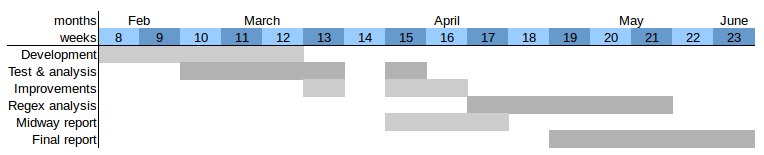
\includegraphics[width=550pt]{GanttDiagram.png}}
	
\newpage

\bibliographystyle{plain}
\nocite{*}
\bibliography{litterature}

\end{document}
